% ============================================================================
% EICL - LAB-001 | Levantamiento y configuración del firewall FortiGate 50E
% Documento fuente independiente, compatible con pdfLaTeX / Overleaf
% Versión 1.2 | 25 de octubre de 2026 (re-saneamiento D-021 de la v1.0)
% Estilo visual alineado con el documento técnico LAB-001 y el documento maestro
% ChkTeX: las advertencias 1, 8 y 13 generan falsos positivos con
% comandos válidos, códigos de activos, fechas y rangos.
% chktex-file 1
% chktex-file 8
% chktex-file 13
% ============================================================================
\documentclass[11pt,a4paper]{article}
% Compila con pdfLaTeX o XeLaTeX.
\usepackage{iftex}
\ifPDFTeX
  \usepackage[utf8]{inputenc}
  \usepackage[T1]{fontenc}
\else
  \usepackage{fontspec}
\fi
% Español: con babel-spanish instalado se usan las opciones de siempre; si falta, babel carga el idioma desde sus .ini.
\IfFileExists{spanish.ldf}
  {\usepackage[spanish,es-nodecimaldot]{babel}}
  {\usepackage{babel}\babelprovide[import,main]{spanish}}
\ifPDFTeX\IfFileExists{lmodern.sty}{\usepackage{lmodern}}{}\fi
\usepackage[margin=2.25cm,headheight=18pt,footskip=28pt]{geometry}
\usepackage[table]{xcolor}
\usepackage{booktabs,tabularx,longtable,array,multirow}
\usepackage{graphicx}
\usepackage{hyperref}
\usepackage{fancyhdr}
\usepackage{titlesec}
\usepackage{enumitem}
\usepackage{lastpage}
\usepackage{listings}
% Sin lmodern las fuentes T1 son de mapa de bits y microtype no puede expandirlas.
\ifPDFTeX\IfFileExists{lmodern.sty}{\usepackage{microtype}}{\usepackage[expansion=false]{microtype}}\else\usepackage{microtype}\fi
\usepackage{ragged2e}
\usepackage{needspace}
\usepackage{etoolbox}

% --- Paleta LAB-001 ---
\definecolor{navy}{HTML}{14283F}
\definecolor{blue}{HTML}{16608B}
\definecolor{muted}{HTML}{5D6977}
\definecolor{light}{HTML}{EAF0F4}
\definecolor{accent}{HTML}{16A3A1}
\definecolor{warning}{HTML}{955A0D}
\definecolor{line}{HTML}{D4DFE6}
\definecolor{white}{HTML}{FFFFFF}

% --- Ajustes generales ---
\setlength{\parindent}{0pt}
\setlength{\parskip}{5pt}
\setlength{\emergencystretch}{2em}
\setlength{\tabcolsep}{4pt}
\renewcommand{\arraystretch}{1.16}
\setlist[itemize]{leftmargin=*,topsep=2pt,itemsep=1pt,parsep=0pt}
\setlist[enumerate]{leftmargin=*,topsep=2pt,itemsep=1pt,parsep=0pt}
\setlist[description]{leftmargin=*,labelindent=0pt,labelsep=0pt,style=nextline,font=\color{navy}\bfseries,topsep=3pt,itemsep=3pt}
\newcolumntype{P}[1]{>{\RaggedRight\arraybackslash}p{#1}}
\newcolumntype{Y}{>{\RaggedRight\arraybackslash}X}
\newcommand{\pc}{\textcolor{warning}{\textbf{[POR CONFIRMAR]}}}
\newcommand{\tech}[1]{\textbf{#1}}
\newcommand{\klabel}[1]{\textcolor{navy}{\textbf{#1}}}
\newcommand{\separador}{\par\vspace{3pt}{\color{line}\hrule height 0.6pt}\vspace{6pt}}
% Estados: COMPLETADA en verde azulado, PENDIENTE en ámbar, el resto en azul marino
\newcommand{\estado}[1]{%
  \ifstrequal{#1}{COMPLETADA}{\textcolor{accent}{\textbf{#1}}}{%
  \ifstrequal{#1}{PENDIENTE}{\textcolor{warning}{\textbf{#1}}}{%
  \textcolor{navy}{\textbf{#1}}}}}

% --- Títulos ---
\titleformat{\section}{\Large\bfseries\color{navy}}{\thesection}{0.7em}{}
\titleformat{\subsection}{\large\bfseries\color{blue}}{\thesubsection}{0.6em}{}
\titleformat{\subsubsection}{\normalsize\bfseries\color{navy}}{\thesubsubsection}{0.5em}{}
\titlespacing*{\section}{0pt}{17pt}{6pt}
\titlespacing*{\subsection}{0pt}{11pt}{4pt}
\titlespacing*{\subsubsection}{0pt}{8pt}{3pt}
\hypersetup{colorlinks=true,linkcolor=blue,urlcolor=blue,pdftitle={EICL - LAB-001 Levantamiento y configuracion del FortiGate 50E},pdfsubject={Firewall FortiGate 50E: recuperacion, configuracion base y evidencias},pdfauthor={Carlos Eduardo Abundis Lira}}

% --- Encabezado y pie ---
\pagestyle{fancy}
\fancyhf{}
\fancyhead[L]{\footnotesize\color{navy}\textbf{EICL} \,|\, LAB-001 \,|\, FortiGate 50E}
\fancyhead[R]{\footnotesize\color{muted} Versión 1.2 \,|\, 25/10/2026}
\fancyfoot[L]{\footnotesize\color{muted} Portafolio técnico \,|\, Información saneada}
\fancyfoot[R]{\footnotesize\color{navy} Página \thepage\ de \pageref{LastPage}}
\renewcommand{\headrulewidth}{0.4pt}
\renewcommand{\footrulewidth}{0pt}
\fancypagestyle{plain}{\pagestyle{fancy}}

% --- Código y bloques monoespaciados ---
\lstdefinestyle{eicl}{
  basicstyle=\ttfamily\footnotesize,
  backgroundcolor=\color{light},
  frame=single,framerule=0.35pt,rulecolor=\color{line},
  breaklines=true,columns=fullflexible,keepspaces=true,
  showstringspaces=false,tabsize=2,
  xleftmargin=7pt,xrightmargin=5pt,
  aboveskip=8pt,belowskip=8pt
}
\lstset{style=eicl}

% --- Recuadros ligeros, sin dependencias especiales ---
\newcommand{\notebox}[2]{%
  \par\smallskip\noindent
  \fcolorbox{line}{light}{\begin{minipage}{0.956\linewidth}
   \vspace{5pt}\textcolor{navy}{\textbf{\MakeUppercase{#1}}}\par\vspace{2pt}#2\vspace{4pt}
  \end{minipage}}\par\smallskip
}
\newcommand{\alertbox}[2]{%
  \par\smallskip\noindent
  \fcolorbox{warning}{light}{\begin{minipage}{0.956\linewidth}
   \vspace{5pt}\textcolor{warning}{\textbf{\MakeUppercase{#1}}}\par\vspace{2pt}#2\vspace{4pt}
  \end{minipage}}\par\smallskip
}

\begin{document}
\hypersetup{pageanchor=false}
% ============================================================================
% PORTADA
% ============================================================================
\begin{titlepage}
\thispagestyle{empty}
\vspace*{1.3cm}
{\color{accent}\rule{2.4cm}{4pt}}\par\vspace{1.1cm}
{\small\bfseries\color{blue} ENTERPRISE INFRASTRUCTURE \& CYBERSECURITY LAB}\par\vspace{0.5cm}
{\Huge\bfseries\color{navy} LAB-001\\[3pt]Levantamiento y configuración\\[3pt]del firewall FortiGate 50E}\par\vspace{0.55cm}
{\Large\color{muted} Memoria técnica | Recuperación, configuración base\\y evidencias de validación}\par
\vspace{1.0cm}
{\color{line}\rule{\textwidth}{0.8pt}}\par\vspace{0.65cm}
\begin{tabularx}{\textwidth}{@{}P{4.2cm}Y@{}}
\textbf{Identificador} & EICL-LAB-001 (componente firewall) \\
\textbf{Versión} & 1.2 \\
\textbf{Fecha} & 25 de octubre de 2026 (contenido técnico al 23/10/2026) \\
\textbf{Responsable} & Carlos Eduardo Abundis Lira \\
\textbf{Equipo} & FortiGate 50E (\texttt{FGT-LAB-01}), FortiOS 6.x \\
\textbf{Estado} & En curso: configuración base validada; integración con el Huawei pendiente \\
\textbf{Clasificación} & Portafolio técnico | Información saneada \\
\end{tabularx}
\vfill
\notebox{Finalidad del documento}{Registrar el estado inicial del firewall, las decisiones de diseño, la configuración aplicada paso a paso y la evidencia de validación, desde la recuperación de un equipo de segunda mano con credenciales desconocidas hasta dejarlo listo para recibir el switch Huawei S5735.}
\vspace{0.35cm}
{\small\color{muted} Referencia de control: EICL-LAB-001 \quad | \quad Documento vivo, sujeto a actualización}\par
\end{titlepage}

% ============================================================================
% PRELIMINARES
% ============================================================================
\hypersetup{pageanchor=true}
\pagenumbering{roman}
\section*{Control del documento}
\addcontentsline{toc}{section}{Control del documento}
{\small\noindent
\begin{tabularx}{\textwidth}{@{}P{3.4cm}Y@{}}
\toprule
\rowcolor{light}\textbf{Campo} & \textbf{Contenido}\\\midrule
Nombre & LAB-001 -- Levantamiento y configuración del FortiGate 50E \\
Proyecto & EICL -- Enterprise Infrastructure \& Cybersecurity Lab \\
Alcance & Firewall FortiGate 50E: recuperación de acceso, reset de fábrica, interfaces, VLAN, DHCP, políticas y administración \\
Versión & 1.2 \\
Fecha & 25/10/2026 (re-saneamiento); contenido técnico al 23/10/2026 \\
Estado & En curso \\
\bottomrule
\end{tabularx}\par}

\subsection*{Historial de versiones}
{\small\noindent
\begin{tabularx}{\textwidth}{@{}P{1.6cm}P{2.2cm}Y@{}}
\toprule
\rowcolor{light}\textbf{Versión} & \textbf{Fecha} & \textbf{Cambio}\\\midrule
1.0 & 23/10/2026 & Versión inicial: levantamiento, pasos 0 a 8 de configuración y evidencias. \\
1.2 & 25/10/2026 & Re-saneamiento para publicación (D-021) en los tres canales: texto, comandos y salidas de consola, e imágenes. Se generalizan la versión exacta de FortiOS y la de BIOS (texto, E-01, E-02 y E-19), se sustituye la sección de datos sensibles por la tabla «Protección de la información» de tres columnas y se añade la nota sobre el estado posterior. Sin cambios técnicos. Se numera 1.2 porque la 1.1 corresponde a una revisión interna no publicada. \\
\bottomrule
\end{tabularx}\par}

\notebox{Estado posterior a este documento}{Este documento conserva el estado del componente al 23/10/2026. El 24/10/2026 se cerraron el respaldo de la configuración y las validaciones que aquí aparecen como pendientes, y se aplicaron cambios al FortiGate (NTP en modo servidor solo en VLAN10-MGMT, filtro de registros en memoria y política 5 hacia SW-LAB-02). Esos cambios y sus evidencias están en las memorias del switch Huawei S5735 (componente B) y del Omada ES208G (componente C).}

\subsection*{Criterios de evidencia}
\begin{itemize}
  \item \textbf{Confirmado:} observado en consola o prueba, con captura (identificador E-xx).
  \item \textbf{Reportado por el operador:} prueba realizada y comunicada, sin captura adjunta.
  \item \textbf{[POR CONFIRMAR]:} dato desconocido o pendiente de verificación.
\end{itemize}

\clearpage
\tableofcontents
\clearpage
\pagenumbering{arabic}



% =====================================================================
\section{Objetivo}

Este documento registra el levantamiento y la configuración base del firewall FortiGate 50E del laboratorio, desde la recuperación de un equipo de segunda mano con credenciales desconocidas hasta dejarlo listo para recibir el switch Huawei S5735. Forma parte del proyecto LAB-001.

\subsection*{Ficha del proyecto LAB-001 --- Infraestructura física y red empresarial base}
{\small\noindent
\begin{tabularx}{\linewidth}{@{}P{4.2cm}Y@{}}
\toprule
\rowcolor{light}\textbf{Campo} & \textbf{Contenido}\\\midrule
Objetivo & Construir desde cero una red de laboratorio físicamente organizada, segmentada y administrable. \\
Tecnologías & Ethernet, Huawei VRP, FortiOS, VLAN, trunking, routing, NAT, DHCP y direccionamiento IPv4. \\
Equipo existente & FortiGate 50E, Huawei S5735-L8P4S-A1, Omada, rack, cableado y router doméstico. \\
Por conseguir & No se ha identificado hardware adicional obligatorio, sujeto a revisión física. \\
Dificultad & Intermedia. \\
Dependencias & Recepción y validación de firewall, switch y cableado. \\
Resultado esperado & Rack organizado, tabla de puertos, topología física y lógica, segmentación por VLAN, routing configurado, acceso a internet desde VLAN autorizadas, aislamiento de tráfico y configuraciones respaldadas. \\
Entregables & LAB-001-Architecture.md, LAB-001-VLAN-Plan.md, LAB-001-Port-Mapping.md, LAB-001-Implementation.md y LAB-001-Validation.md. Este documento cubre la parte del firewall. \\
\bottomrule
\end{tabularx}\par}

\subsection{Alcance de este documento}

\begin{description}
  \item[Incluye] Recuperación de acceso, reset de fábrica, levantamiento del hardware y del software, identidad y hora, puertos físicos, red de emergencia (OOB), WAN, DNS, NTP, subinterfaces VLAN, DHCP, objetos, políticas de firewall y restricción de la administración.
  \item[No incluye] Configuración del Huawei S5735, del Omada y del TL-SG108, la red de los hipervisores ni la validación de punta a punta con equipos conectados a las VLAN. Esas actividades se documentarán al completarse.
\end{description}

\subsection{Estado del componente}

{\small\noindent
\begin{tabularx}{\linewidth}{@{}P{1.4cm}YP{2.9cm}@{}}
\toprule
\rowcolor{light}\textbf{Paso} & \textbf{Actividad} & \textbf{Estado}\\\midrule
0 & Recuperación de acceso y reset de fábrica & \estado{COMPLETADA} \\
1 & Hostname y zona horaria & \estado{COMPLETADA} \\
2--3 & Identificación de puertos y liberación de \texttt{lan5} & \estado{COMPLETADA} \\
4 & Red de emergencia OOB en \texttt{lan} & \estado{COMPLETADA} \\
5 & WAN, ruta por defecto, DNS y NTP & \estado{COMPLETADA} \\
6 & Subinterfaces VLAN y DHCP & \estado{COMPLETADA} \\
7 & Objetos y políticas de firewall & \estado{COMPLETADA} \\
8 & Trusted hosts y administración desde la PC & \estado{COMPLETADA} \\
-- & Respaldo de la configuración & \estado{PENDIENTE} \\
-- & Validación de punta a punta con el Huawei conectado & \estado{PENDIENTE} \\
\bottomrule
\end{tabularx}\par}

% =====================================================================
\section{Arquitectura}

\subsection{Topología}

El laboratorio queda detrás de dos redes domésticas: la del módem del proveedor y la del router del cuarto. La WAN del FortiGate se conecta al router del cuarto y todo el laboratorio vive en las VLAN internas.

\begin{lstlisting}
Internet
   |
Modem ISP 192.168.0.1 -- (red de casa 192.168.0.0/24)
   |
Router del cuarto TP-Link Archer C3200 192.168.1.1 -- (red del cuarto 192.168.1.0/24)
   |                                                    `-- PC de escritorio <IP-PC-ADMIN>
[wan1] FortiGate 50E 192.168.1.2  -- [lan1-lan4] OOB 10.10.254.1/24 (emergencia)
   |
[lan5] trunk 802.1Q (VLAN 10, 20, 30, 40, 50)
   |
Huawei S5735 GE0/0/1 (pendiente de configurar)
\end{lstlisting}

\subsection{Plan de VLAN}

Rango del laboratorio: \texttt{10.10.0.0/16}, con el tercer octeto igual al ID de VLAN.

{\small\noindent
\begin{tabularx}{\linewidth}{@{}P{1.3cm}P{2.3cm}P{2.6cm}P{2.1cm}Y@{}}
\toprule
\rowcolor{light}\textbf{VLAN} & \textbf{Interfaz} & \textbf{Subred} & \textbf{Gateway} & \textbf{DHCP y uso}\\\midrule
10 & VLAN10-MGMT & 10.10.10.0/24 & 10.10.10.1 & .100--.120. Gestión de firewall, switches e hipervisores. \\
20 & VLAN20-SRV & 10.10.20.0/24 & 10.10.20.1 & .100--.199. VM de servicios. \\
30 & VLAN30-MON & 10.10.30.0/24 & 10.10.30.1 & Sin DHCP (IP fijas). Monitoreo y SOC. \\
40 & VLAN40-DMZ & 10.10.40.0/24 & 10.10.40.1 & Sin DHCP (IP fijas). Servicios publicados. \\
50 & VLAN50-LAB & 10.10.50.0/24 & 10.10.50.1 & .100--.199. Pruebas y clientes. \\
-- & lan (OOB) & 10.10.254.0/24 & 10.10.254.1 & .100--.110. Acceso de emergencia, sin salida a internet. \\
\bottomrule
\end{tabularx}\par}

Reservadas, sin crear todavía: VLAN 60 (respaldos, LAB-008) y VLAN 70 (clúster Proxmox, LAB-012). La VLAN 999 (nativa de trunks y puertos sin uso) se configura en los switches, no en el FortiGate.

\subsection{Convención de direcciones dentro de cada /24}

{\small\noindent
\begin{tabularx}{\linewidth}{@{}P{2.5cm}Y@{}}
\toprule
\rowcolor{light}\textbf{Rango} & \textbf{Uso}\\\midrule
.1 & Gateway (FortiGate) \\
.2--.9 & Equipos de red, IP fija configurada en el equipo \\
.10--.49 & Servidores e hipervisores, IP fija configurada en el equipo \\
.50--.99 & Reservado \\
.100--.199 & DHCP: laptops, VM de prueba y equipos temporales \\
.200--.254 & Reservado \\
\bottomrule
\end{tabularx}\par}

\subsection{Asignación de puertos del FortiGate}

{\small\noindent
\begin{tabularx}{\linewidth}{@{}P{2.2cm}P{3cm}P{3.6cm}Y@{}}
\toprule
\rowcolor{light}\textbf{Puerto} & \textbf{Función} & \textbf{Conecta a} & \textbf{Configuración}\\\midrule
wan1 & WAN (WAN-CUARTO) & Archer C3200 & 192.168.1.2/24, gateway 192.168.1.1 \\
wan2 & Reservado & -- & Apagado (\texttt{status down}) \\
lan1--lan4 & OOB & Laptop de emergencia & Interfaz \texttt{lan}, 10.10.254.1/24 \\
lan5 & Trunk 802.1Q & Huawei GE0/0/1 & Subinterfaces VLAN 10--50 \\
modem & Sin uso & -- & Valores de fábrica \\
fortilink & Sin uso & -- & Valores de fábrica (no aplica al Huawei) \\
\bottomrule
\end{tabularx}\par}

\subsection{Matriz de políticas (semana 1)}

Origen en las filas, destino en las columnas. Sí: permitido. No: denegado. Esp.: solo puertos específicos, a definir en LAB-004 a LAB-007.

{\footnotesize\noindent
\begin{tabularx}{\linewidth}{@{}P{2.3cm}YYYYYYY@{}}
\toprule
\rowcolor{light}\textbf{Origen} & \textbf{MGMT} & \textbf{SRV} & \textbf{MON} & \textbf{DMZ} & \textbf{LAB} & \textbf{Internet} & \textbf{Casa\slash cuarto}\\\midrule
MGMT & -- & Sí & Sí & Sí & Sí & Sí & No \\
SRV & No & -- & Esp. & No & No & Sí & No \\
MON & Esp. & Esp. & -- & Esp. & Esp. & Sí & No \\
DMZ & No & No & Esp. & -- & No & Sí & No \\
LAB & No & No & No & Esp. & -- & Sí & No \\
PC escritorio & 443, 22, 8006 & No & No & No & No & -- & -- \\
\bottomrule
\end{tabularx}\par}

En la semana 1 solo se configuran los permisos «Sí» y los bloqueos; los «Esp.» quedan denegados por la regla implícita hasta su proyecto.

\subsection{Decisiones de diseño}

\begin{description}
  \item[Rango 10.10.0.0/16] Evita choques con la red de casa (192.168.0.0/24), la del cuarto (192.168.1.0/24) y Tailscale (100.64.0.0/10).
  \item[Router-on-a-stick] El FortiGate rutea entre todas las VLAN, de modo que todo el tráfico entre segmentos pasa por políticas y queda registrado. El Huawei se queda en capa 2.
  \item[WAN hacia el router del cuarto] La red doméstica queda arriba, el laboratorio abajo, y el laboratorio nunca entrega DHCP hacia arriba.
  \item[MON-SOC separada de MGMT] El monitoreo recibe tráfico de todos los segmentos; separarlo evita abrir la red de administración a redes menos confiables (mínimo privilegio).
  \item[Dominio interno] \texttt{eicl.internal}; el sufijo \texttt{.internal} está reservado para uso privado.
  \item[IP fijas para infraestructura] Servidores, hipervisores y switches usan IP fija configurada en el equipo; DHCP solo para equipos temporales. MON-SOC y DMZ no tienen DHCP.
  \item[Puerto OOB] \texttt{lan1}--\texttt{lan4} quedan como red de emergencia para recuperar el acceso si falla la configuración de VLAN.
  \item[Administración desde la PC] Excepción acotada a una sola IP de origen (la PC de administración; IP redactada en este documento), solo hacia MGMT y solo por 443, 22 y 8006.
\end{description}

\subsection{Limitaciones conocidas}

\begin{itemize}
  \item \textbf{Triple NAT} (proveedor, router del cuarto y FortiGate): la salida a internet funciona; las VPN y la publicación de servicios requerirán más trabajo (NAT-T en IPsec).
  \item \textbf{Sin FortiGuard}: las bases de antivirus e IPS son de 2015. Firewall, NAT, ruteo y VPN funcionan; antivirus, IPS y filtro web no.
  \item \textbf{Sin disco de logs} (\texttt{Log hard disk: Not available}): los logs viven en memoria. Se resolverá con syslog externo en LAB-006.
\end{itemize}

% =====================================================================
\section{Prerrequisitos y levantamiento inicial}

\subsection{Entorno}

{\small\noindent
\begin{tabularx}{\linewidth}{@{}P{4.2cm}Y@{}}
\toprule
\rowcolor{light}\textbf{Campo} & \textbf{Contenido}\\\midrule
Red de casa & Módem del proveedor en 192.168.0.1 (192.168.0.0/24). \\
Red del cuarto & TP-Link Archer C3200 en 192.168.1.1 (192.168.1.0/24); pool DHCP 192.168.1.100--.199. \\
PC de administración & Windows, conectada por cable al Archer; IP fija reservada por MAC en el Archer (redactada en este documento). \\
IP de la WAN & 192.168.1.2, fuera del pool DHCP; se comprobó libre con ping antes de asignarla. \\
Acceso de consola & Cable de consola y MobaXterm, 9600 baudios, 8 bits, sin paridad, 1 bit de parada, sin control de flujo. \\
\bottomrule
\end{tabularx}\par}

\newpage
\subsection{Levantamiento del equipo}

Datos tomados de \texttt{get system status} tras el reset de fábrica (evidencias E-01, E-02 y E-19).

{\small\noindent
\begin{tabularx}{\linewidth}{@{}P{4.2cm}Y@{}}
\toprule
\rowcolor{light}\textbf{Campo} & \textbf{Contenido}\\\midrule
Modelo & FortiGate 50E \\
Número de serie & \texttt{FGT50EXXXXXXXXXX} (enmascarado salvo el prefijo del modelo; el completo vive solo en el inventario privado) \\
System Part-Number & P17464-05 \\
BIOS & \texttt{<REDACTADO>} (consta en el inventario privado) \\
FortiOS & 6.x, versión GA (versión exacta y build omitidos en la publicación) \\
Virus-DB & 1.00123 (2015-12-11) \\
Extended DB & 1.00000 (2018-04-09) \\
IPS-DB & 6.00741 (2015-12-01) \\
IPS-ETDB & 0.00000 (2001-01-01) \\
APP-DB & 6.00741 (2015-12-01) al inicio; 37.00317 (2026-10-22) tras tener salida a internet \\
INDUSTRIAL-DB & 6.00741 (2015-12-01) \\
Botnet DB & 1.00000 (2012-05-28) \\
Disco de logs & No disponible \\
Modo de operación & NAT \\
VDOM & Desactivados (máximo 5) \\
HA & Standalone \\
FIPS-CC & Desactivado \\
Hora al inicio & 17:50:58, unos 50 minutos de atraso respecto a la hora real \\
Licencia y registro en FortiCare & \pc \\
\bottomrule
\end{tabularx}\par}

\subsection{Estado previo al reset}

El equipo llegó con la configuración de una institución anterior: hostname institucional (anonimizado en este documento) y credenciales de administrador desconocidas. La configuración previa no se respaldó a propósito, porque podía contener direcciones, VPN o datos ajenos.

\subsection{Configuración de fábrica observada tras el reset}

Evidencias E-03 a E-07.

{\footnotesize\noindent
\begin{tabularx}{\linewidth}{@{}P{2cm}P{2.3cm}P{3cm}Y@{}}
\toprule
\rowcolor{light}\textbf{Interfaz} & \textbf{Tipo} & \textbf{IP} & \textbf{Observaciones}\\\midrule
wan1 & physical & DHCP & \texttt{allowaccess ping fgfm}, rol wan \\
wan2 & physical & DHCP & \texttt{allowaccess ping fgfm}, rol wan \\
modem & physical & PPPoE & Para módem USB 3G/4G \\
ssl.root & tunnel & -- & Interfaz de la VPN SSL \\
lan & hard-switch & 192.168.1.99/24 & lan1--lan5 sobre \texttt{sw0}; \texttt{allowaccess ping https ssh http fgfm fabric}; STP activo \\
fortilink & hard-switch & 169.254.1.1/24 & Gestión de FortiSwitch; LLDP activo \\
\bottomrule
\end{tabularx}\par}

\begin{itemize}
  \item \textbf{DHCP 1}: en \texttt{lan}, rango 192.168.1.110--.210, gateway 192.168.1.99.
  \item \textbf{DHCP 2}: en \texttt{fortilink}, rango 169.254.1.2--.254, solo para FortiSwitch y FortiExtender.
  \item \textbf{Política 1}: \texttt{lan} \textrightarrow{} \texttt{wan1}, origen, destino y servicio \texttt{all}, accept, con NAT.
\end{itemize}

\alertbox{Traslape con la red del cuarto}{La red de fábrica de \texttt{lan} (192.168.1.99/24) usa el mismo segmento que la red del cuarto. Por eso se cambió \texttt{lan} antes de configurar la WAN, y nunca se conectó un puerto interno del FortiGate al Archer.}

% =====================================================================
\section{Implementación}

\subsection{Cronología}

Horas locales aproximadas (UTC-6), tomadas del registro de la sesión de trabajo.

{\small\noindent
\begin{tabularx}{\linewidth}{@{}P{2cm}Y@{}}
\toprule
\rowcolor{light}\textbf{Hora} & \textbf{Evento}\\\midrule
18:17 & Se detecta que el FortiGate tiene contraseña de administrador desconocida. \\
18:21 & Primer intento con la cuenta \texttt{maintainer}: \texttt{Login incorrect}. \\
18:31 & Acceso con \texttt{maintainer} tras un apagado físico. \\
18:36 & \texttt{execute factoryreset} en curso. \\
18:41 & Primer \texttt{get system status} con el equipo limpio. \\
19:23 & Paso 1 validado (hostname y hora). \\
20:15--20:31 & Pasos 4 y 5 validados (OOB, WAN, DNS, NTP). \\
20:41 & Zona horaria corregida a Central America. \\
20:57 & Paso 6 validado (subinterfaces VLAN y DHCP). \\
21:23 & Paso 7 validado (objetos y políticas). \\
21:32 & Paso 8 validado (trusted hosts y administración desde la PC). \\
21:37 & NTP sincronizado con desfase menor a 0.1 s. \\
\bottomrule
\end{tabularx}\par}

\subsection{Paso 0: recuperación de acceso y reset de fábrica}

Se usó la cuenta de recuperación \texttt{maintainer}, que solo funciona por consola y durante una ventana corta después de un arranque en frío.

\begin{enumerate}
  \item Consola abierta en MobaXterm (9600 8N1).
  \item Desconectar y reconectar la corriente del equipo (un reinicio por software no sirve).
  \item En cuanto aparece \texttt{login:}, usuario \texttt{maintainer} y contraseña \texttt{bcpb} seguida del número de serie con letras en mayúsculas, pegada desde un bloc de notas.
  \item Ya dentro, ejecutar el reset de fábrica.
  \item Primer acceso con \texttt{admin} sin contraseña y creación de una contraseña nueva, guardada en el gestor de contraseñas.
\end{enumerate}

\begin{lstlisting}
execute factoryreset
\end{lstlisting}

\alertbox{Acción destructiva}{\texttt{execute factoryreset} borra toda la configuración. Se ejecutó sin respaldo de forma intencional, porque la configuración pertenecía a la institución anterior.}

\newpage
\subsection{Paso 1: identidad y hora}

El hostname identifica al equipo en el prompt, los logs, el syslog y el monitoreo. La hora correcta es necesaria para correlacionar eventos, para los certificados HTTPS y para IPsec. Zona horaria final: \texttt{07}, Central America (GMT-6 sin horario de verano).

\begin{lstlisting}
config system global
    set hostname FGT-LAB-01
    set timezone 07
end
execute time 19:23:00
\end{lstlisting}

\subsection{Pasos 2 y 3: identificación de puertos y liberación de lan5}

Se identificaron los puertos con estos comandos y se sacó \texttt{lan5} del switch interno para usarlo como trunk:

\begin{itemize}
  \item \texttt{get system interface physical}
  \item \texttt{show system virtual-switch}
  \item \texttt{show system interface}
\end{itemize}

\begin{lstlisting}
config system virtual-switch
    edit "lan"
        config port
            delete "lan5"
        end
    next
end
\end{lstlisting}

\subsection{Paso 4: red de emergencia OOB}

Se borró la política de fábrica (salida sin restricciones de \texttt{lan} a \texttt{wan1}), se movió \texttt{lan} a 10.10.254.1/24 y se ajustó su DHCP. \texttt{allowaccess} reemplaza la lista completa, así que se eliminaron \texttt{http}, \texttt{fgfm} y \texttt{fabric}.

\begin{lstlisting}
config firewall policy
    delete 1
end
config system interface
    edit "lan"
        set alias "OOB"
        set ip 10.10.254.1 255.255.255.0
        set allowaccess ping https ssh
    next
end
config system dhcp server
    edit 1
        set default-gateway 10.10.254.1
        set netmask 255.255.255.0
        config ip-range
            edit 1
                set start-ip 10.10.254.100
                set end-ip 10.10.254.110
            next
        end
    next
end
\end{lstlisting}

\subsection{Paso 5: WAN, ruta por defecto, DNS y NTP}

\begin{lstlisting}
config system interface
    edit "wan1"
        set alias "WAN-CUARTO"
        set mode static
        set ip 192.168.1.2 255.255.255.0
        set allowaccess ping
    next
end
config router static
    edit 1
        set gateway 192.168.1.1
        set device "wan1"
    next
end
config system dns
    set primary 1.1.1.1
    set secondary 8.8.8.8
end
config system ntp
    set ntpsync enable
    set type custom
    config ntpserver
        edit 1
            set server "pool.ntp.org"
        next
    end
end
\end{lstlisting}

Conexión física: un solo cable de \texttt{wan1} a un puerto LAN del Archer C3200. En el paso 8 se amplió \texttt{allowaccess} de \texttt{wan1}.

\subsection{Paso 6: subinterfaces VLAN y DHCP}

Cinco subinterfaces sobre \texttt{lan5}. Solo MGMT permite administración (\texttt{https ssh}); las demás solo responden \texttt{ping}.

\begin{lstlisting}
config system interface
    edit "VLAN10-MGMT"
        set vdom "root"
        set interface "lan5"
        set vlanid 10
        set ip 10.10.10.1 255.255.255.0
        set allowaccess ping https ssh
        set role lan
    next
    edit "VLAN20-SRV"
        set vdom "root"
        set interface "lan5"
        set vlanid 20
        set ip 10.10.20.1 255.255.255.0
        set allowaccess ping
        set role lan
    next
    edit "VLAN30-MON"
        set vdom "root"
        set interface "lan5"
        set vlanid 30
        set ip 10.10.30.1 255.255.255.0
        set allowaccess ping
        set role lan
    next
    edit "VLAN40-DMZ"
        set vdom "root"
        set interface "lan5"
        set vlanid 40
        set ip 10.10.40.1 255.255.255.0
        set allowaccess ping
        set role dmz
    next
    edit "VLAN50-LAB"
        set vdom "root"
        set interface "lan5"
        set vlanid 50
        set ip 10.10.50.1 255.255.255.0
        set allowaccess ping
        set role lan
    next
end
\end{lstlisting}

DHCP para MGMT, SRV y LAB (el ID del servidor coincide con la VLAN). \texttt{dns-service default} entrega como DNS los mismos servidores del FortiGate.

\begin{lstlisting}
config system dhcp server
    edit 10
        set interface "VLAN10-MGMT"
        set default-gateway 10.10.10.1
        set netmask 255.255.255.0
        set dns-service default
        set domain "eicl.internal"
        config ip-range
            edit 1
                set start-ip 10.10.10.100
                set end-ip 10.10.10.120
            next
        end
    next
    edit 20
        set interface "VLAN20-SRV"
        set default-gateway 10.10.20.1
        set netmask 255.255.255.0
        set dns-service default
        set domain "eicl.internal"
        config ip-range
            edit 1
                set start-ip 10.10.20.100
                set end-ip 10.10.20.199
            next
        end
    next
    edit 50
        set interface "VLAN50-LAB"
        set default-gateway 10.10.50.1
        set netmask 255.255.255.0
        set dns-service default
        set domain "eicl.internal"
        config ip-range
            edit 1
                set start-ip 10.10.50.100
                set end-ip 10.10.50.199
            next
        end
    next
end
\end{lstlisting}

\subsection{Paso 7: objetos y políticas de firewall}

Se apagó \texttt{wan2} (puerto sin uso) y se crearon objetos con nombre para que las reglas se lean solas.

\begin{lstlisting}
config system interface
    edit "wan2"
        set status down
    next
end
config firewall address
    edit "NET-CASA"
        set subnet 192.168.0.0 255.255.255.0
    next
    edit "NET-CUARTO"
        set subnet 192.168.1.0 255.255.255.0
    next
    edit "NET-MGMT"
        set subnet 10.10.10.0 255.255.255.0
    next
    edit "PC-ADMIN-ESCRITORIO"
        set subnet <IP-PC-ADMIN> 255.255.255.255
    next
end
config firewall addrgrp
    edit "GRP-REDES-DOMESTICAS"
        set member "NET-CASA" "NET-CUARTO"
    next
end
config firewall service custom
    edit "SVC-PROXMOX-WEB"
        set tcp-portrange 8006
    next
end
\end{lstlisting}

{\footnotesize\noindent
\begin{tabularx}{\linewidth}{@{}P{0.6cm}P{3.3cm}P{3.1cm}P{3cm}P{1.8cm}Y@{}}
\toprule
\rowcolor{light}\textbf{\#} & \textbf{Nombre} & \textbf{Origen} & \textbf{Destino} & \textbf{Servicio} & \textbf{Acción}\\\midrule
1 & DENY-LAB-A-CASA & VLAN 10--50, all & wan1, GRP-REDES-DOMESTICAS & ALL & deny \\
2 & LAB-A-INTERNET & VLAN 10--50, all & wan1, all & ALL & accept, NAT \\
3 & MGMT-A-INTERNAS & VLAN10-MGMT, NET-MGMT & VLAN 20--50, all & ALL & accept \\
4 & PC-ADMIN-A-MGMT & wan1, PC-ADMIN-ESCRITORIO & VLAN10-MGMT, NET-MGMT & HTTPS, SSH, 8006 & accept \\
\bottomrule
\end{tabularx}\par}

\begin{lstlisting}
config firewall policy
    edit 1
        set name "DENY-LAB-A-CASA"
        set srcintf "VLAN10-MGMT" "VLAN20-SRV" "VLAN30-MON" "VLAN40-DMZ" "VLAN50-LAB"
        set dstintf "wan1"
        set srcaddr "all"
        set dstaddr "GRP-REDES-DOMESTICAS"
        set action deny
        set schedule "always"
        set service "ALL"
        set logtraffic all
    next
    edit 2
        set name "LAB-A-INTERNET"
        set srcintf "VLAN10-MGMT" "VLAN20-SRV" "VLAN30-MON" "VLAN40-DMZ" "VLAN50-LAB"
        set dstintf "wan1"
        set srcaddr "all"
        set dstaddr "all"
        set action accept
        set schedule "always"
        set service "ALL"
        set nat enable
        set logtraffic all
    next
    edit 3
        set name "MGMT-A-INTERNAS"
        set srcintf "VLAN10-MGMT"
        set dstintf "VLAN20-SRV" "VLAN30-MON" "VLAN40-DMZ" "VLAN50-LAB"
        set srcaddr "NET-MGMT"
        set dstaddr "all"
        set action accept
        set schedule "always"
        set service "ALL"
        set logtraffic all
    next
    edit 4
        set name "PC-ADMIN-A-MGMT"
        set srcintf "wan1"
        set dstintf "VLAN10-MGMT"
        set srcaddr "PC-ADMIN-ESCRITORIO"
        set dstaddr "NET-MGMT"
        set action accept
        set schedule "always"
        set service "HTTPS" "SSH" "SVC-PROXMOX-WEB"
        set logtraffic all
    next
end
\end{lstlisting}

\notebox{Reglas aplicadas al escribir políticas}{El sentido lo define quien inicia la conexión; las respuestas regresan solas porque el firewall es \emph{stateful}. Las reglas deben ser lo más específicas posible. Lo que no está permitido queda denegado por la regla implícita. El orden importa: el FortiGate aplica la primera regla que coincide, por eso el bloqueo hacia las redes domésticas va antes de la salida a internet.}

\notebox{Concesiones temporales}{El servicio \texttt{ALL} en la política 2 es temporal para la semana 1; en LAB-004 se limitará a HTTP/HTTPS, DNS, NTP y ping.}

\subsection{Paso 8: restricción de la administración}

Las políticas controlan el tráfico \emph{a través} del FortiGate; el acceso \emph{al} FortiGate lo controlan \texttt{allowaccess} y los \emph{trusted hosts}. La consola no se ve afectada por los trusted hosts.

\begin{lstlisting}
config system admin
    edit "admin"
        set trusthost1 <IP-PC-ADMIN> 255.255.255.255
        set trusthost2 10.10.10.0 255.255.255.0
        set trusthost3 10.10.254.0 255.255.255.0
    next
end
config system interface
    edit "wan1"
        set allowaccess ping https ssh
    next
end
\end{lstlisting}

\alertbox{Administración en la WAN}{Habilitar HTTPS y SSH en \texttt{wan1} solo es aceptable aquí porque esa WAN está dentro de la red del cuarto, detrás de dos NAT, y los trusted hosts limitan el acceso a una IP. En una WAN expuesta a internet no se habilita.}

% =====================================================================
\section{Validación}

\subsection{Pruebas realizadas}

{\footnotesize\noindent
\begin{tabularx}{\linewidth}{@{}P{1cm}YP{3.2cm}P{1.8cm}P{2.9cm}@{}}
\toprule
\rowcolor{light}\textbf{Paso} & \textbf{Prueba} & \textbf{Resultado} & \textbf{Evidencia} & \textbf{Estado}\\\midrule
1 & \texttt{get system status}: hostname y hora & FGT-LAB-01, 19:23:03 & E-02 & \estado{COMPLETADA} \\
3 & \texttt{lan5} fuera del switch interno & lan1--lan4 en \texttt{lan}; lan5 independiente & E-08, E-09 & \estado{COMPLETADA} \\
4 & Configuración de \texttt{lan} OOB, DHCP y políticas & 10.10.254.1/24; .100--.110; sin políticas & E-10 a E-12 & \estado{COMPLETADA} \\
4 & Laptop en \texttt{lan1}: DHCP, ping y acceso web & IP recibida, ping y HTTPS correctos & Reportado por el operador & \estado{COMPLETADA} \\
5 & Ping al gateway 192.168.1.1 & 5/5, 0.4 ms promedio & E-13 & \estado{COMPLETADA} \\
5 & Ping a internet 1.1.1.1 & 5/5, 9.3 ms promedio & E-14 & \estado{COMPLETADA} \\
5 & Ping a \texttt{google.com} (DNS) & Resuelve y responde, 9.5 ms & E-15 & \estado{COMPLETADA} \\
5 & Tabla de rutas & \texttt{S* 0.0.0.0/0 via 192.168.1.1, wan1} & E-16 & \estado{COMPLETADA} \\
5 & Ping desde la PC a 192.168.1.2 & 4/4, TTL 255 & E-18 & \estado{COMPLETADA} \\
5 & Sincronización NTP & Offset de -0.05 s tras corregir la zona horaria & E-17, E-19, E-28 & \estado{COMPLETADA} \\
6 & Subinterfaces VLAN 10--50 & 5 interfaces tipo vlan con su IP & E-20 & \estado{COMPLETADA} \\
6 & DHCP 10, 20 y 50 & Gateway, rango y dominio correctos & E-21 & \estado{COMPLETADA} \\
7 & \texttt{wan2} apagado & \texttt{status: down} & E-22 & \estado{COMPLETADA} \\
7 & Objetos, grupo y servicio & 4 objetos, 1 grupo, 1 servicio & E-23 a E-25 & \estado{COMPLETADA} \\
7 & Orden y contenido de políticas & 1, 2, 3, 4; NAT solo en la 2 & E-26 & \estado{COMPLETADA} \\
8 & Trusted hosts y \texttt{allowaccess} de wan1 & Tres trusted hosts; ping https ssh & E-27 & \estado{COMPLETADA} \\
8 & HTTPS y SSH desde la PC a 192.168.1.2 & Acceso correcto & Reportado por el operador & \estado{COMPLETADA} \\
8 & Prueba negativa desde un celular en la red del cuarto & Acceso rechazado & Reportado por el operador & \estado{COMPLETADA} \\
\bottomrule
\end{tabularx}\par}

\notebox{Estado «up» en interfaces}{En \texttt{get system interface}, \texttt{status: up} indica que la interfaz está habilitada administrativamente, no que tenga cable o tráfico. Las subinterfaces VLAN aparecen \texttt{up} aunque \texttt{lan5} no tiene cable todavía.}

\subsection{Validaciones pendientes}

{\small\noindent
\begin{tabularx}{\linewidth}{@{}YP{2.9cm}@{}}
\toprule
\rowcolor{light}\textbf{Prueba} & \textbf{Estado}\\\midrule
Un equipo en cada VLAN con DHCP recibe IP, alcanza su gateway y sale a internet & \estado{PENDIENTE} \\
Desde las VLAN no se alcanza 192.168.1.0/24 ni 192.168.0.0/24 (política 1) & \estado{PENDIENTE} \\
SRV no alcanza MGMT y MGMT sí alcanza SRV & \estado{PENDIENTE} \\
La PC alcanza el Proxmox en MGMT con la ruta estática \texttt{route -p add 10.10.0.0 mask 255.255.0.0 192.168.1.2} & \estado{PENDIENTE} \\
Revisión de logs y contadores por política & \estado{PENDIENTE} \\
\texttt{show full-configuration firewall policy 1} muestra \texttt{set action deny} & \estado{PENDIENTE} \\
\bottomrule
\end{tabularx}\par}

% =====================================================================
\section{Troubleshooting}

{\footnotesize\noindent
\begin{tabularx}{\linewidth}{@{}P{3.2cm}YY@{}}
\toprule
\rowcolor{light}\textbf{Síntoma} & \textbf{Causa} & \textbf{Solución}\\\midrule
\texttt{Login incorrect} con \texttt{maintainer} y contraseña de longitud correcta & La ventana de acceso de \texttt{maintainer} había vencido; requiere arranque en frío reciente. & Apagado físico, contraseña lista para pegar y login inmediato al ver \texttt{login:}. \\
\texttt{Unknown action 0} en \texttt{get system status} dentro de la sesión \texttt{maintainer} & No determinada: el sistema seguía arrancando (\texttt{System is starting...}) o la sesión tenía comandos limitados. Se descartaron los VDOM porque \texttt{config global} tampoco funcionó. & Se ejecutó directamente \texttt{execute factoryreset}, que sí funcionó. \\
\texttt{command parse error before 'global'} en \texttt{config system global} y \texttt{config global} & Misma sesión limitada que el caso anterior. & Resuelto con el reset de fábrica. \\
Offset NTP de 3600 s exactos & Causa probable: la zona horaria elegida al inicio aplicaba horario de verano (número de zona inicial \pc), y el reloj interno (UTC) quedó una hora desfasado. & Zona \texttt{07} Central America, sin \texttt{execute time} posterior; offset final de -0.05 s. \\
\texttt{command parse error} o \texttt{Unmatched double quote} & Errores de tecleo o comillas sin cerrar. & FortiOS rechaza el comando sin aplicar cambios; se repite la línea correcta. \\
\texttt{set action deny} no aparece en \texttt{show} & \texttt{show} omite los valores por defecto, y la acción por defecto de una política es \texttt{deny}. & Verificar con \texttt{show full-configuration}. \\
\bottomrule
\end{tabularx}\par}

% =====================================================================
\section{Backup y recuperación}

\subsection{Rutas de recuperación}

\begin{description}
  \item[Puerto OOB] Una laptop en cualquiera de \texttt{lan1} a \texttt{lan4} recibe una IP entre 10.10.254.100 y .110, y entra a la web del FortiGate en 10.10.254.1 por HTTPS, aunque falle la configuración de VLAN.
  \item[Consola] El acceso por cable de consola no depende de los trusted hosts.
  \item[Cuenta maintainer] Disponible por consola tras un arranque en frío, como se usó en el paso 0. Si en el futuro se desactiva por seguridad, esta ruta deja de existir.
\end{description}

\subsection{Respaldo de la configuración}

\estado{PENDIENTE}; ejecución confirmada \pc.

\begin{enumerate}
  \item En \texttt{https://192.168.1.2}, menú \textbf{admin} \textrightarrow{} \textbf{Configuration} \textrightarrow{} \textbf{Backup}.
  \item Destino \textbf{Local PC}; cifrado a elección.
  \item Guardar en una carpeta privada, fuera del repositorio público, con un nombre descriptivo:
\begin{lstlisting}
FGT-LAB-01_2026-10-23_base-LAB-001.conf
\end{lstlisting}
\end{enumerate}

\alertbox{Respaldos y hashes}{Los respaldos de configuración y la salida de \texttt{show system admin} contienen el hash de la contraseña de administrador. No se publican en GitHub.}

% =====================================================================
\section{Lecciones aprendidas}

\begin{itemize}
  \item La cuenta \texttt{maintainer} depende del tiempo: un fallo no significa que esté desactivada. Conviene tener la contraseña lista para pegar.
  \item Un equipo de segunda mano no debe darse por limpio: este llegó con la configuración completa de una institución.
  \item En FortiOS un error de tecleo no rompe nada; lo peligroso es un comando bien escrito con un valor equivocado. Por eso cada paso termina con validación.
  \item \texttt{allowaccess} reemplaza la lista completa; no agrega a la anterior.
  \item \texttt{show} oculta los valores por defecto; \texttt{show full-configuration} los muestra.
  \item El reloj interno funciona en UTC y la zona horaria solo convierte. Una zona con horario de verano desfasa el NTP una hora exacta, y el problema puede reaparecer meses después.
  \item \texttt{status: up} significa habilitada, no conectada.
  \item Los objetos de tipo \texttt{interface-subnet} siguen solos a la subred de su interfaz.
  \item Las pruebas negativas (el celular rechazado) son tan importantes como las positivas.
  \item Las capturas pueden contener datos sensibles (número de serie, hash de contraseña); se revisan antes de publicarlas.
\end{itemize}

% =====================================================================
\appendix
\section{Configuración aplicada consolidada}

Resumen de los cambios respecto a la configuración de fábrica, en orden de aplicación. No incluye contraseñas ni hashes.

\begin{lstlisting}
# Paso 1
config system global
    set hostname FGT-LAB-01
    set timezone 07
end
# Paso 3
config system virtual-switch
    edit "lan"
        config port
            delete "lan5"
        end
    next
end
# Paso 4
config firewall policy
    delete 1
end
config system interface
    edit "lan"
        set alias "OOB"
        set ip 10.10.254.1 255.255.255.0
        set allowaccess ping https ssh
    next
end
config system dhcp server
    edit 1
        set default-gateway 10.10.254.1
        config ip-range
            edit 1
                set start-ip 10.10.254.100
                set end-ip 10.10.254.110
            next
        end
    next
end
# Paso 5 (allowaccess de wan1 ampliado en el paso 8)
config system interface
    edit "wan1"
        set alias "WAN-CUARTO"
        set mode static
        set ip 192.168.1.2 255.255.255.0
        set allowaccess ping https ssh
    next
    edit "wan2"
        set status down
    next
end
config router static
    edit 1
        set gateway 192.168.1.1
        set device "wan1"
    next
end
config system dns
    set primary 1.1.1.1
    set secondary 8.8.8.8
end
config system ntp
    set ntpsync enable
    set type custom
    config ntpserver
        edit 1
            set server "pool.ntp.org"
        next
    end
end
# Paso 6: subinterfaces VLAN10-MGMT ... VLAN50-LAB y DHCP 10, 20, 50
#         (ver seccion de implementacion)
# Paso 7: objetos NET-CASA, NET-CUARTO, NET-MGMT, PC-ADMIN-ESCRITORIO,
#         grupo GRP-REDES-DOMESTICAS, servicio SVC-PROXMOX-WEB,
#         politicas 1 a 4 (ver seccion de implementacion)
# Paso 8
config system admin
    edit "admin"
        set trusthost1 <IP-PC-ADMIN> 255.255.255.255
        set trusthost2 10.10.10.0 255.255.255.0
        set trusthost3 10.10.254.0 255.255.255.0
    next
end
\end{lstlisting}

% =====================================================================
\section{Evidencias}

Capturas de la consola del FortiGate y de la PC de administración. Las capturas están censuradas: número de serie en E-01, E-02 y E-19; versión exacta de FortiOS, build y versión de BIOS en E-01, E-02 y E-19; IP de la PC de administración en E-23 y E-27; hash de la contraseña en E-27; longitud de la contraseña en E-28, y UUID de objetos y políticas en E-07, E-23, E-24 y E-26. No se incluyen las capturas de la sesión \texttt{maintainer} porque muestran el hostname de la institución anterior.

{\footnotesize\noindent
\begin{tabularx}{\linewidth}{@{}P{1.2cm}YP{1.2cm}@{}}
\toprule
\rowcolor{light}\textbf{ID} & \textbf{Contenido} & \textbf{Paso}\\\midrule
E-01 & \texttt{get system status} tras el reset (serial y versiones redactados) & 0 \\
E-02 & Hostname y hora ajustada (serial y versiones redactados) & 1 \\
E-03 & Interfaces físicas de fábrica & 2 \\
E-04 & Switch interno de fábrica (lan1--lan5) & 2 \\
E-05 & \texttt{show system interface} de fábrica & 2 \\
E-06 & DHCP de fábrica & 3 \\
E-07 & Política de fábrica (UUID redactado) & 3 \\
E-08 & Switch interno sin \texttt{lan5} & 3 \\
E-09 & \texttt{lan5} como interfaz independiente & 3 \\
E-10 & Interfaz \texttt{lan} como OOB & 4 \\
E-11 & DHCP de la red OOB & 4 \\
E-12 & Políticas vacías & 4 \\
E-13 & Ping al gateway del cuarto & 5 \\
E-14 & Ping a 1.1.1.1 & 5 \\
E-15 & Ping a \texttt{google.com} & 5 \\
E-16 & Tabla de rutas & 5 \\
E-17 & NTP con offset de 3600 s & 5 \\
E-18 & Ping desde la PC a la WAN & 5 \\
E-19 & Zona horaria 07 y estado del sistema (serial y versiones redactados) & 5 \\
E-20 & Subinterfaces VLAN & 6 \\
E-21 & Servidores DHCP & 6 \\
E-22 & \texttt{wan2} apagado & 7 \\
E-23 & Objetos de dirección (IP de la PC y UUID redactados) & 7 \\
E-24 & Grupo de direcciones (UUID redactados) & 7 \\
E-25 & Servicio SVC-PROXMOX-WEB & 7 \\
E-26 & Políticas 1 a 4 (UUID redactados) & 7 \\
E-27 & Trusted hosts y wan1 (IP de la PC y hash redactados) & 8 \\
E-28 & NTP sincronizado (longitud de la contraseña redactada) & 8 \\
\bottomrule
\end{tabularx}\par}

\par\noindent\begin{minipage}{\linewidth}
\klabel{E-01:} \texttt{get system status} tras el reset de fábrica.\par\vspace{3pt}
\centering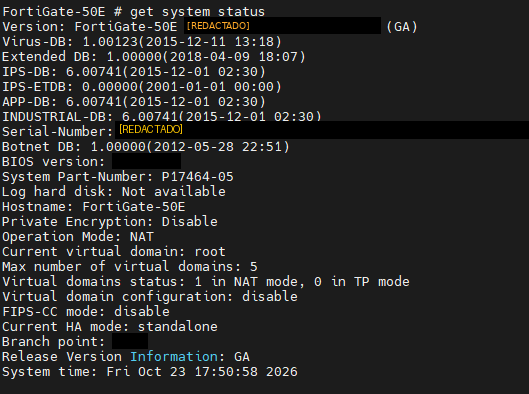
\includegraphics[width=0.6\linewidth]{evidencias/LAB-001-fortigate/E01-status-fabrica.png}
\end{minipage}\par\bigskip

\par\noindent\begin{minipage}{\linewidth}
\klabel{E-02:} hostname \texttt{FGT-LAB-01} y hora ajustada.\par\vspace{3pt}
\centering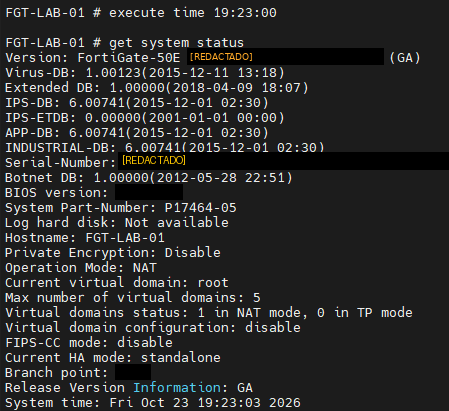
\includegraphics[width=0.6\linewidth]{evidencias/LAB-001-fortigate/E02-status-hostname-hora.png}
\end{minipage}\par\bigskip

\par\noindent\begin{minipage}{\linewidth}
\klabel{E-03:} interfaces físicas de fábrica.\par\vspace{3pt}
\centering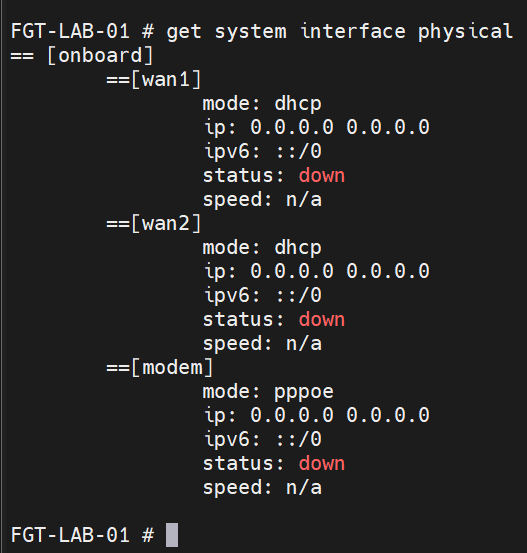
\includegraphics[width=0.5\linewidth]{evidencias/LAB-001-fortigate/E03-interfaces-fisicas-fabrica.png}
\end{minipage}\par\bigskip

\par\noindent\begin{minipage}{\linewidth}
\klabel{E-04:} switch interno de fábrica.\par\vspace{3pt}
\centering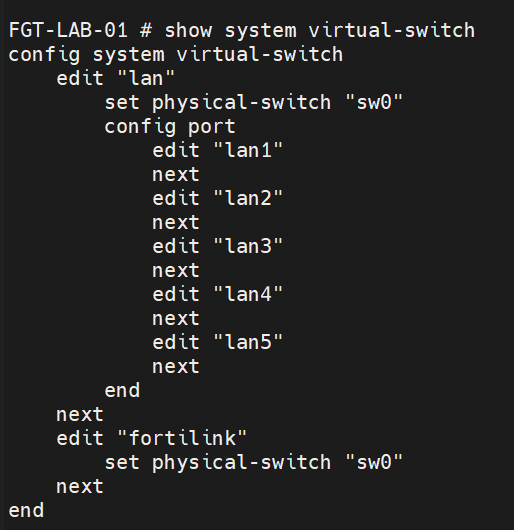
\includegraphics[width=0.5\linewidth]{evidencias/LAB-001-fortigate/E04-virtual-switch-fabrica.png}
\end{minipage}\par\bigskip

\par\noindent\begin{minipage}{\linewidth}
\klabel{E-05:} interfaces de fábrica.\par\vspace{3pt}
\centering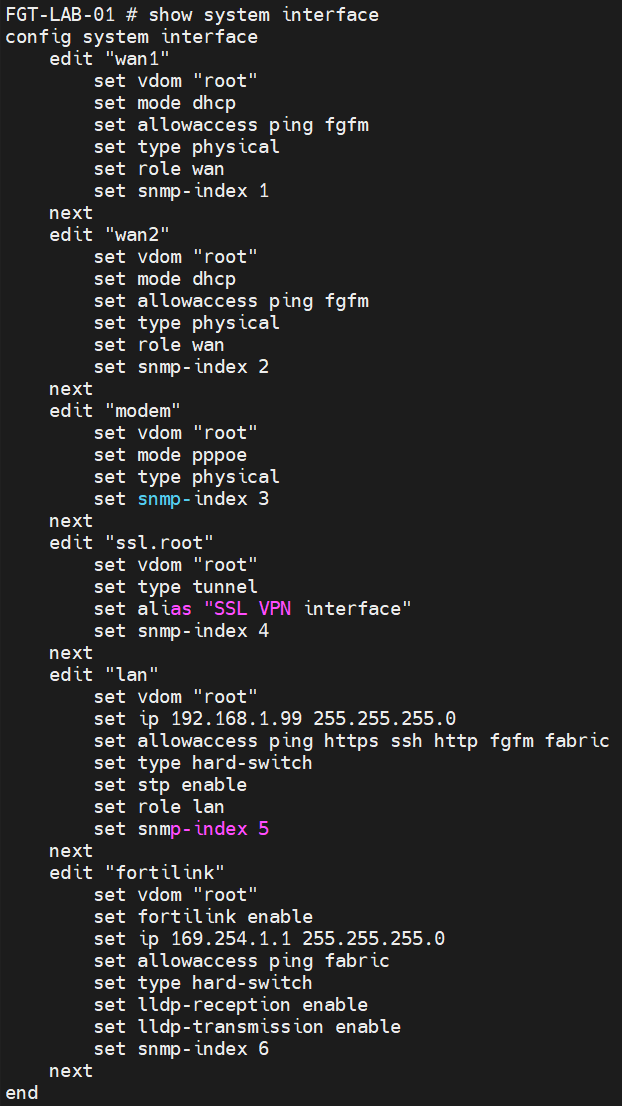
\includegraphics[height=0.75\textheight,width=0.9\linewidth,keepaspectratio]{evidencias/LAB-001-fortigate/E05-interfaces-fabrica.png}
\end{minipage}\par\bigskip

\par\noindent\begin{minipage}{\linewidth}
\klabel{E-06:} DHCP de fábrica.\par\vspace{3pt}
\centering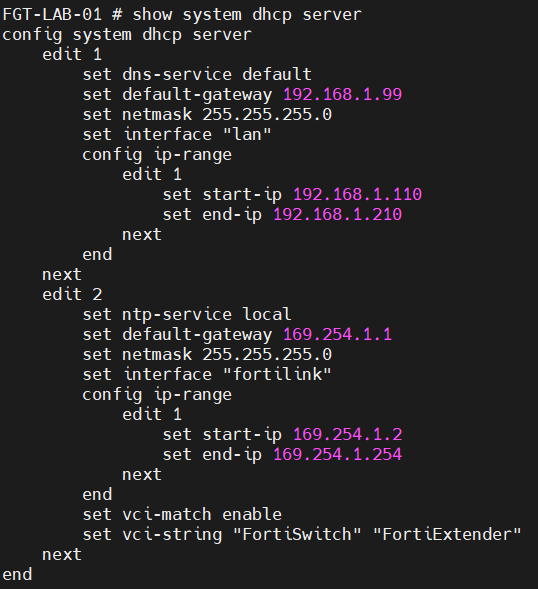
\includegraphics[width=0.6\linewidth]{evidencias/LAB-001-fortigate/E06-dhcp-fabrica.png}
\end{minipage}\par\bigskip

\par\noindent\begin{minipage}{\linewidth}
\klabel{E-07:} política de fábrica.\par\vspace{3pt}
\centering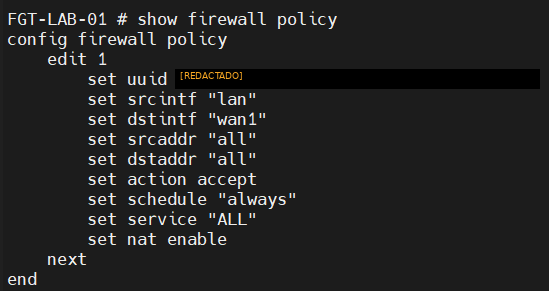
\includegraphics[width=0.6\linewidth]{evidencias/LAB-001-fortigate/E07-politica-fabrica.png}
\end{minipage}\par\bigskip

\par\noindent\begin{minipage}{\linewidth}
\klabel{E-08:} switch interno sin \texttt{lan5}.\par\vspace{3pt}
\centering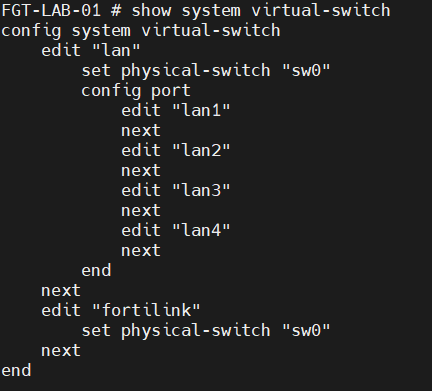
\includegraphics[width=0.5\linewidth]{evidencias/LAB-001-fortigate/E08-virtual-switch-sin-lan5.png}
\end{minipage}\par\bigskip

\par\noindent\begin{minipage}{\linewidth}
\klabel{E-09:} \texttt{lan5} independiente.\par\vspace{3pt}
\centering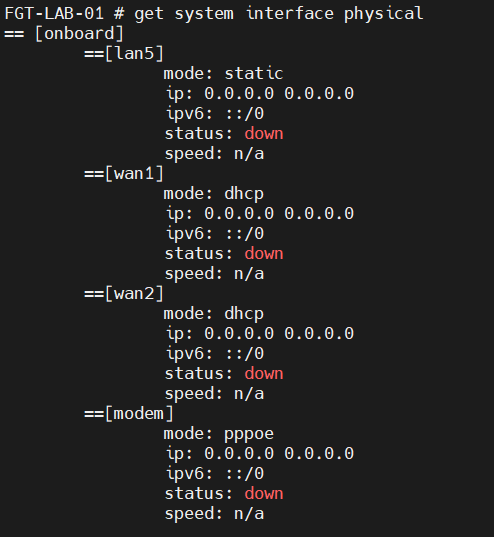
\includegraphics[width=0.5\linewidth]{evidencias/LAB-001-fortigate/E09-lan5-independiente.png}
\end{minipage}\par\bigskip

\par\noindent\begin{minipage}{\linewidth}
\klabel{E-10:} interfaz \texttt{lan} como OOB.\par\vspace{3pt}
\centering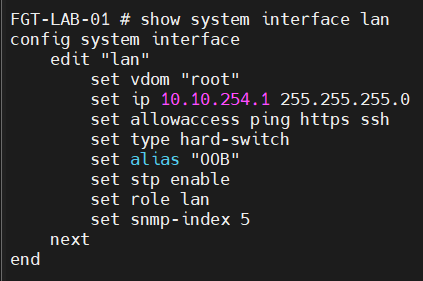
\includegraphics[width=0.5\linewidth]{evidencias/LAB-001-fortigate/E10-lan-oob.png}
\end{minipage}\par\bigskip

\par\noindent\begin{minipage}{\linewidth}
\klabel{E-11:} DHCP de la red OOB.\par\vspace{3pt}
\centering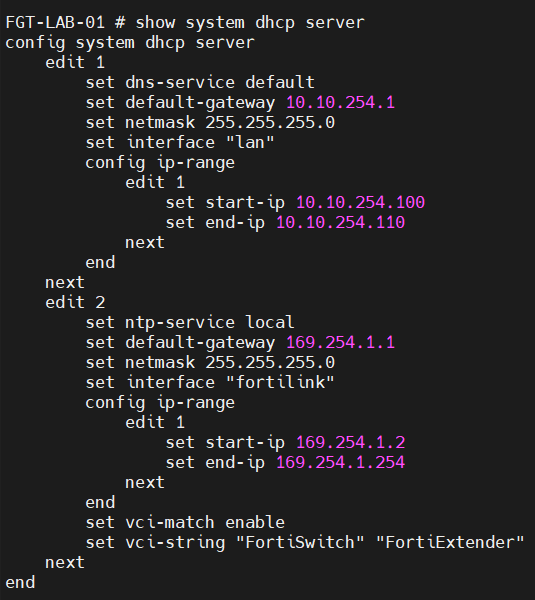
\includegraphics[width=0.6\linewidth]{evidencias/LAB-001-fortigate/E11-dhcp-oob.png}
\end{minipage}\par\bigskip

\par\noindent\begin{minipage}{\linewidth}
\klabel{E-12:} políticas vacías.\par\vspace{3pt}
\centering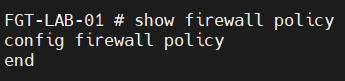
\includegraphics[width=0.4\linewidth]{evidencias/LAB-001-fortigate/E12-politicas-vacias.png}
\end{minipage}\par\bigskip

\par\noindent\begin{minipage}{\linewidth}
\klabel{E-13:} ping al gateway del cuarto.\par\vspace{3pt}
\centering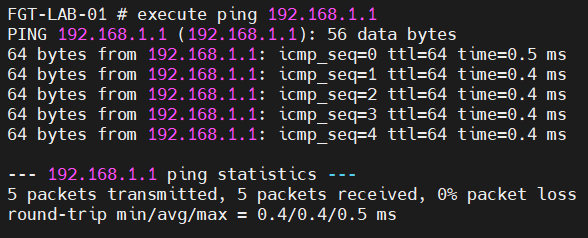
\includegraphics[width=0.7\linewidth]{evidencias/LAB-001-fortigate/E13-ping-gateway.png}
\end{minipage}\par\bigskip

\par\noindent\begin{minipage}{\linewidth}
\klabel{E-14:} ping a 1.1.1.1.\par\vspace{3pt}
\centering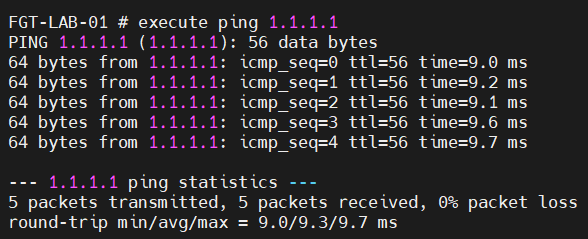
\includegraphics[width=0.7\linewidth]{evidencias/LAB-001-fortigate/E14-ping-internet.png}
\end{minipage}\par\bigskip

\par\noindent\begin{minipage}{\linewidth}
\klabel{E-15:} ping a \texttt{google.com}.\par\vspace{3pt}
\centering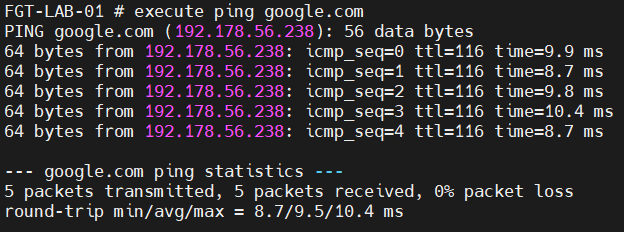
\includegraphics[width=0.7\linewidth]{evidencias/LAB-001-fortigate/E15-ping-dns.png}
\end{minipage}\par\bigskip

\par\noindent\begin{minipage}{\linewidth}
\klabel{E-16:} tabla de rutas.\par\vspace{3pt}
\centering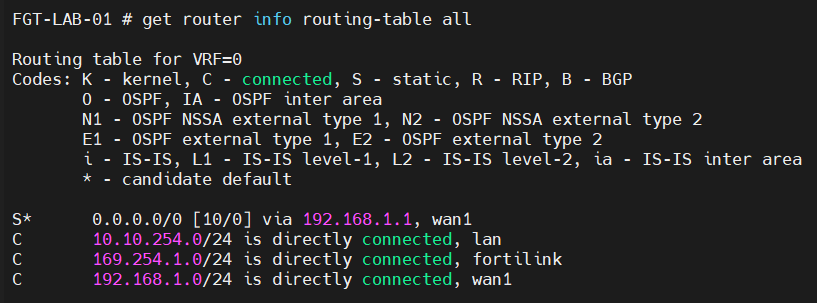
\includegraphics[width=0.9\linewidth]{evidencias/LAB-001-fortigate/E16-tabla-rutas.png}
\end{minipage}\par\bigskip

\par\noindent\begin{minipage}{\linewidth}
\klabel{E-17:} NTP con offset de 3600 s.\par\vspace{3pt}
\centering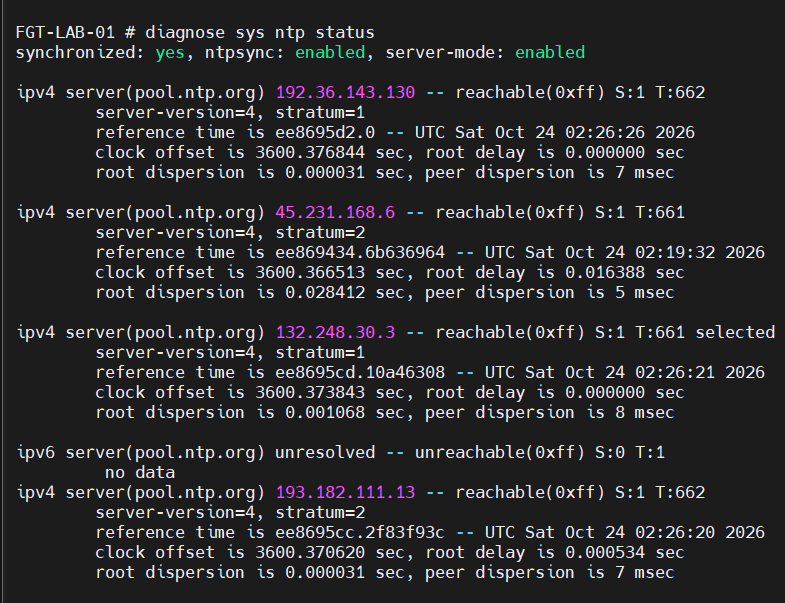
\includegraphics[width=0.9\linewidth]{evidencias/LAB-001-fortigate/E17-ntp-offset-3600.png}
\end{minipage}\par\bigskip

\par\noindent\begin{minipage}{\linewidth}
\klabel{E-18:} ping desde la PC de administración a la WAN.\par\vspace{3pt}
\centering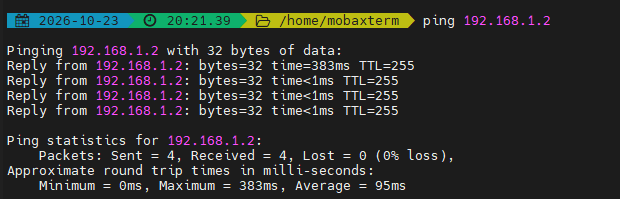
\includegraphics[width=0.7\linewidth]{evidencias/LAB-001-fortigate/E18-ping-pc-a-wan.png}
\end{minipage}\par\bigskip

\par\noindent\begin{minipage}{\linewidth}
\klabel{E-19:} zona horaria 07, estado del sistema y NTP antes de la corrección.\par\vspace{3pt}
\centering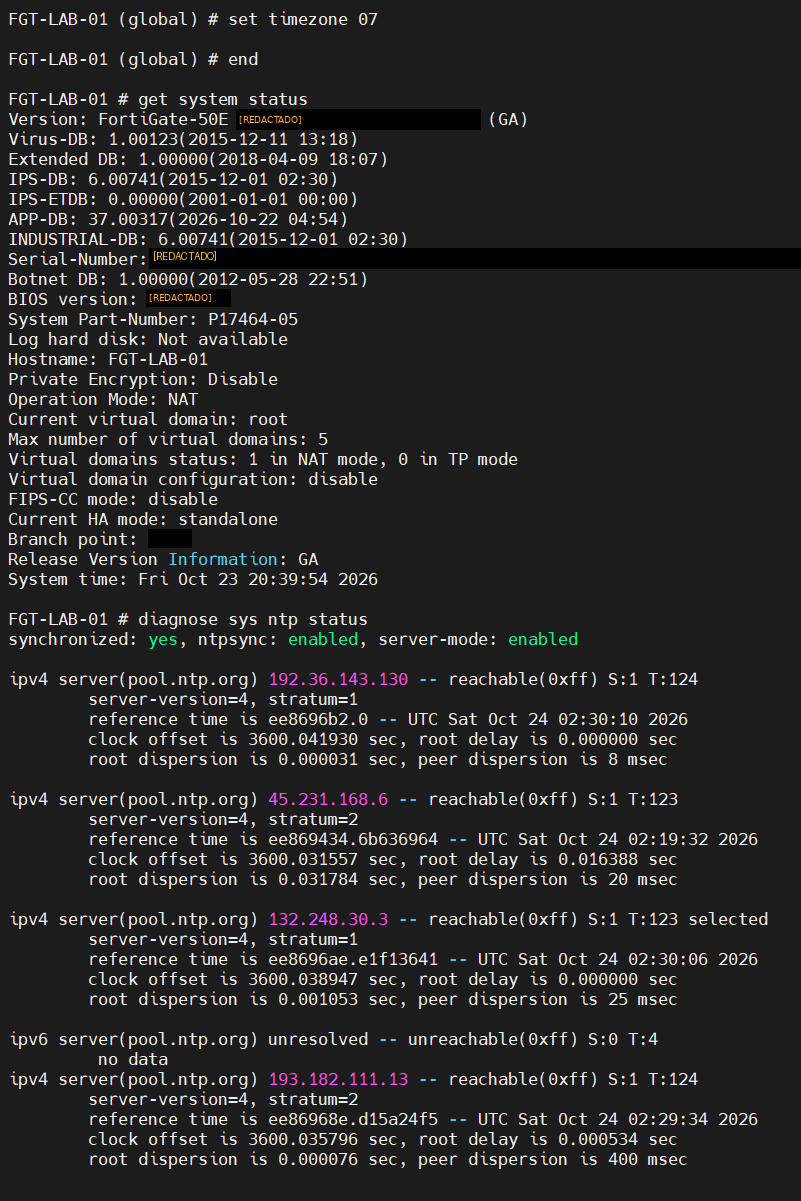
\includegraphics[height=0.8\textheight,width=0.9\linewidth,keepaspectratio]{evidencias/LAB-001-fortigate/E19-zona-horaria-status.png}
\end{minipage}\par\bigskip

\par\noindent\begin{minipage}{\linewidth}
\klabel{E-20:} subinterfaces VLAN.\par\vspace{3pt}
\centering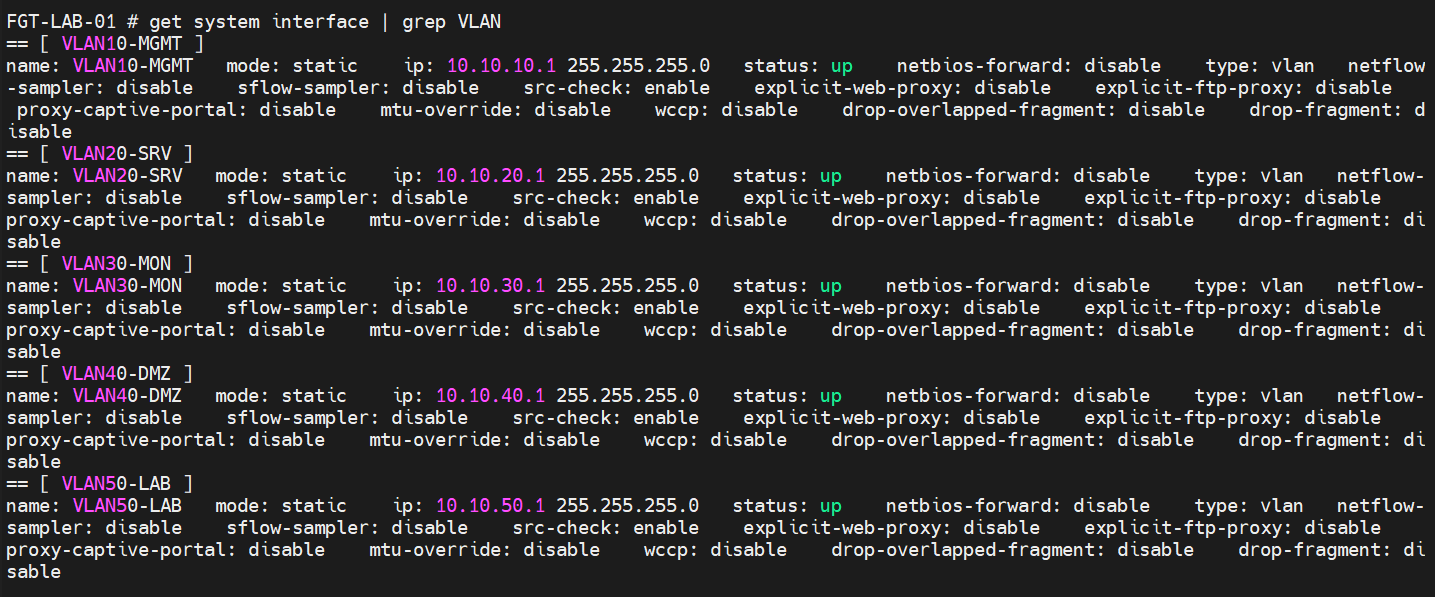
\includegraphics[width=\linewidth]{evidencias/LAB-001-fortigate/E20-subinterfaces-vlan.png}
\end{minipage}\par\bigskip

\par\noindent\begin{minipage}{\linewidth}
\klabel{E-21:} servidores DHCP.\par\vspace{3pt}
\centering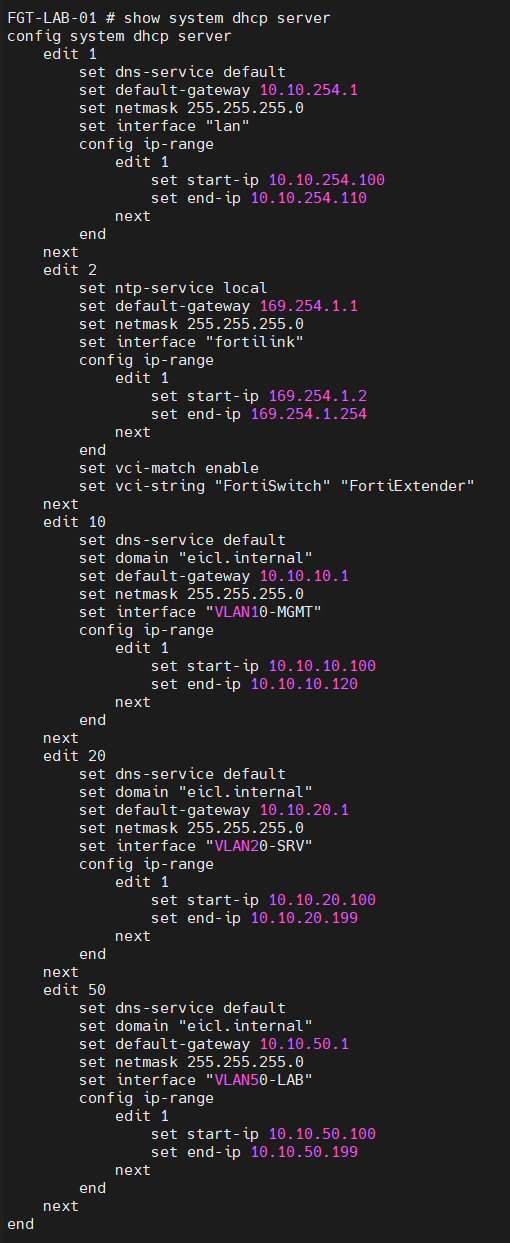
\includegraphics[height=0.8\textheight,width=0.9\linewidth,keepaspectratio]{evidencias/LAB-001-fortigate/E21-dhcp-vlans.png}
\end{minipage}\par\bigskip

\par\noindent\begin{minipage}{\linewidth}
\klabel{E-22:} \texttt{wan2} apagado.\par\vspace{3pt}
\centering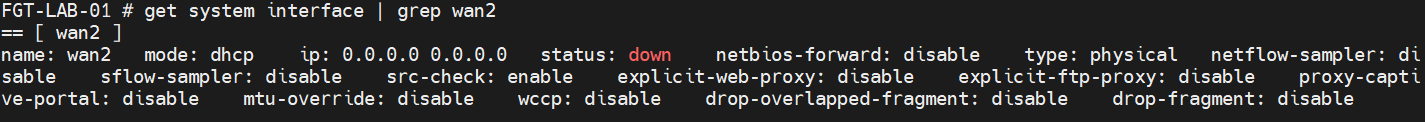
\includegraphics[width=\linewidth]{evidencias/LAB-001-fortigate/E22-wan2-down.png}
\end{minipage}\par\bigskip

\par\noindent\begin{minipage}{\linewidth}
\klabel{E-23:} objetos de dirección.\par\vspace{3pt}
\centering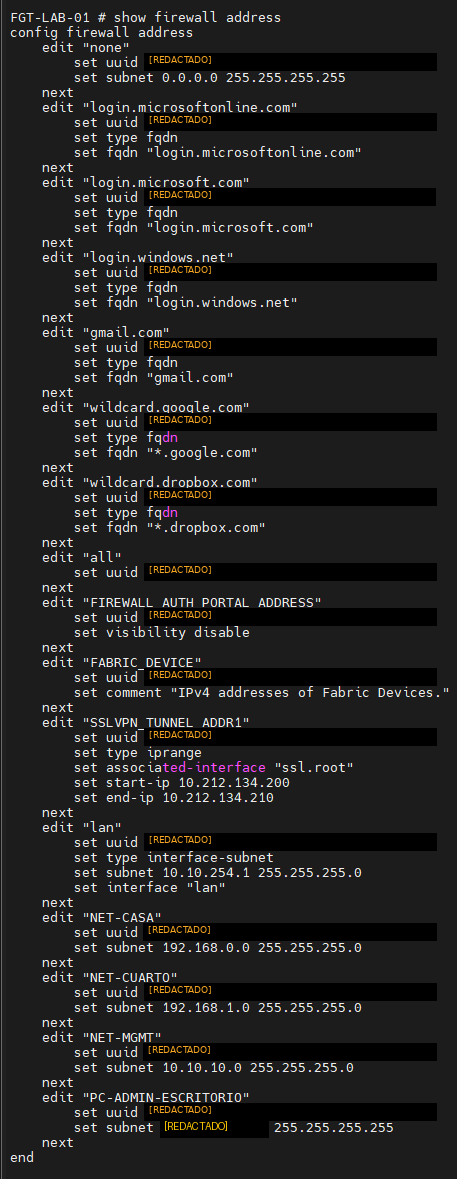
\includegraphics[height=0.8\textheight,width=0.9\linewidth,keepaspectratio]{evidencias/LAB-001-fortigate/E23-objetos-direccion.png}
\end{minipage}\par\bigskip

\par\noindent\begin{minipage}{\linewidth}
\klabel{E-24:} grupo de direcciones.\par\vspace{3pt}
\centering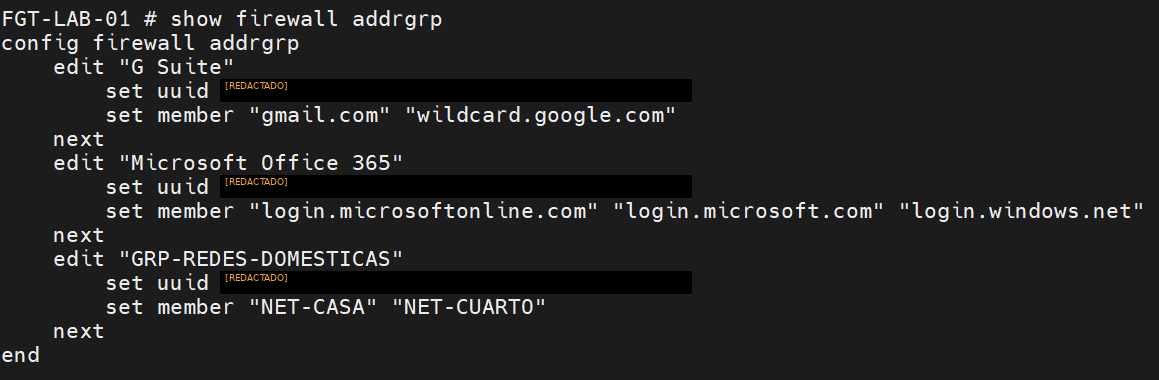
\includegraphics[width=0.9\linewidth]{evidencias/LAB-001-fortigate/E24-grupo-direcciones.png}
\end{minipage}\par\bigskip

\par\noindent\begin{minipage}{\linewidth}
\klabel{E-25:} servicio SVC-PROXMOX-WEB.\par\vspace{3pt}
\centering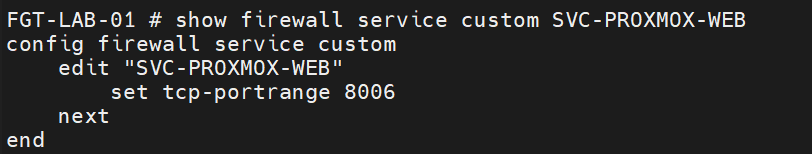
\includegraphics[width=0.7\linewidth]{evidencias/LAB-001-fortigate/E25-servicio-proxmox.png}
\end{minipage}\par\bigskip

\par\noindent\begin{minipage}{\linewidth}
\klabel{E-26:} políticas 1 a 4.\par\vspace{3pt}
\centering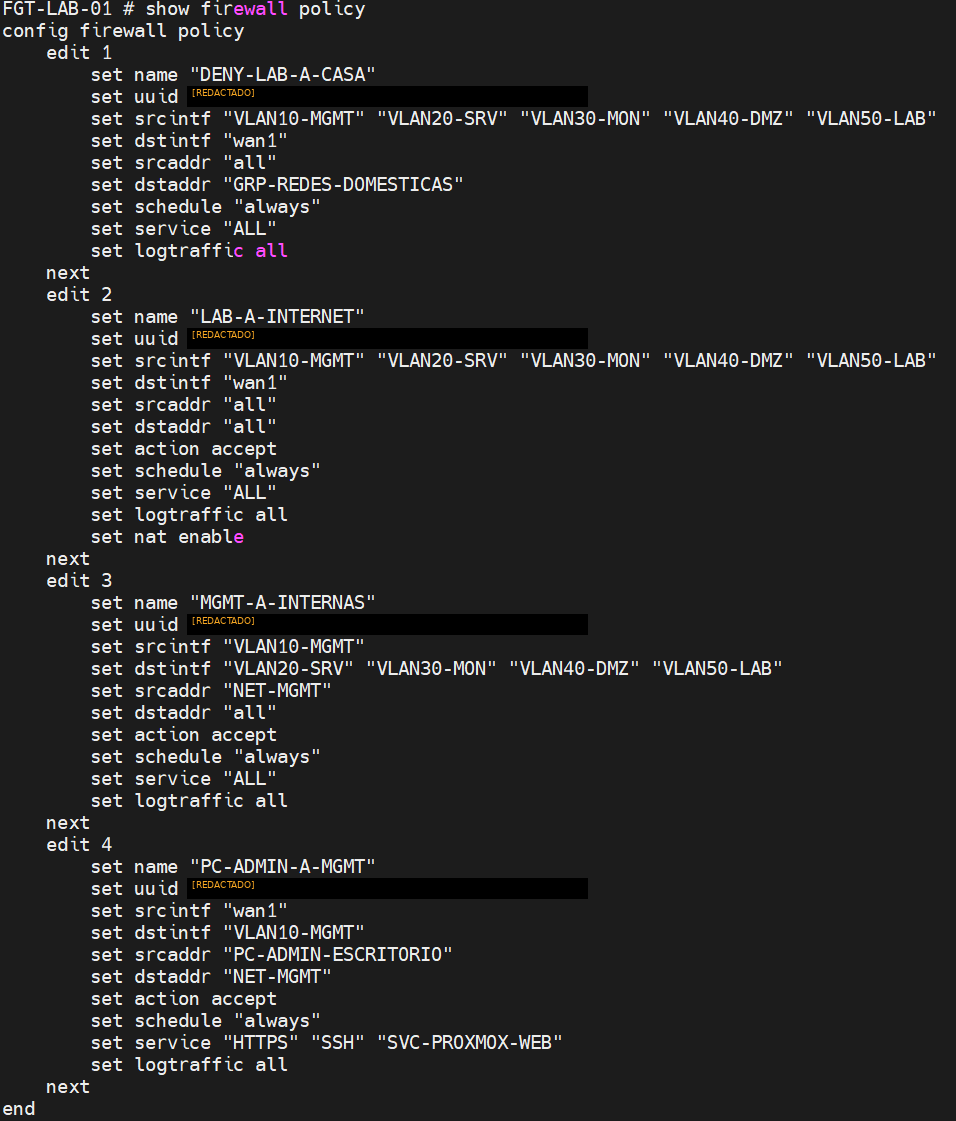
\includegraphics[height=0.8\textheight,width=0.9\linewidth,keepaspectratio]{evidencias/LAB-001-fortigate/E26-politicas.png}
\end{minipage}\par\bigskip

\par\noindent\begin{minipage}{\linewidth}
\klabel{E-27:} trusted hosts y \texttt{wan1}.\par\vspace{3pt}
\centering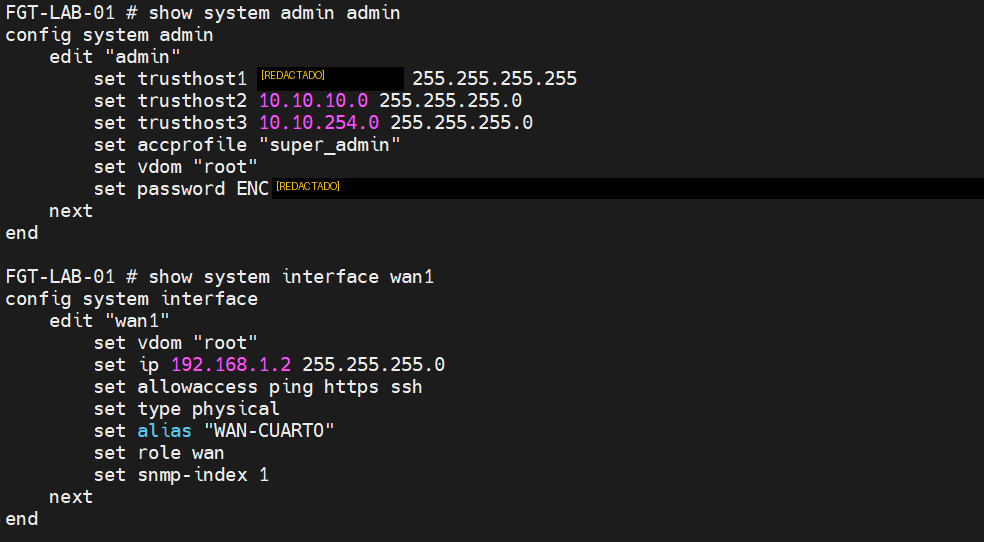
\includegraphics[width=0.9\linewidth]{evidencias/LAB-001-fortigate/E27-trusted-hosts-wan1.png}
\end{minipage}\par\bigskip

\par\noindent\begin{minipage}{\linewidth}
\klabel{E-28:} NTP sincronizado.\par\vspace{3pt}
\centering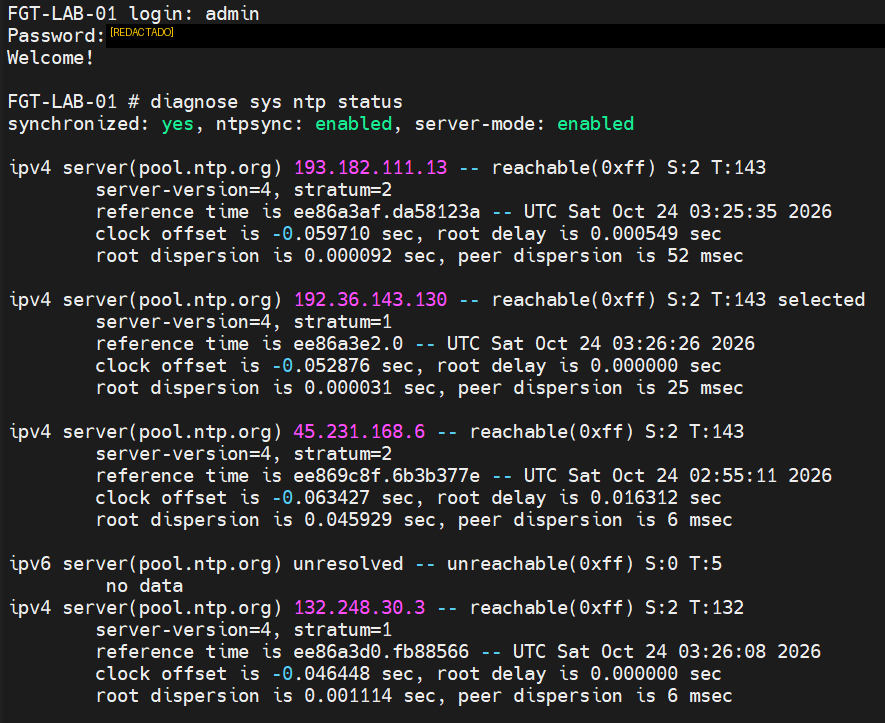
\includegraphics[width=0.8\linewidth]{evidencias/LAB-001-fortigate/E28-ntp-sincronizado.png}
\end{minipage}\par\bigskip

% =====================================================================
\section{Protección de la información}

Criterio del proyecto: se censura cualquier dato que no sea de dominio público o que pueda representar una vulnerabilidad, aunque sea mínima; en caso de duda, se censura. En el texto se usan marcadores (\texttt{<IP-PC-ADMIN>}, \texttt{<REDACTADO>}); en las capturas, recuadros negros opacos, con la etiqueta [REDACTADO] cuando hay espacio. Los originales sin censura solo se guardan en la carpeta privada del operador.

\textbf{Canales revisados en esta versión (1.2):} texto general (incluidos tablas, pies de figura y metadatos del PDF), comandos y salidas de consola en forma de texto (bloques de configuración) e imágenes (las 28 capturas, revisadas completas, incluidos prompts y barras de título).

\subsection*{Datos censurados}
{\small\noindent
\begin{tabularx}{\linewidth}{@{}P{3.4cm}P{6.2cm}Y@{}}
\toprule
\rowcolor{light}\textbf{Dato} & \textbf{Tratamiento (dónde se censuró)} & \textbf{Motivo de protección}\\\midrule
Contraseña de \texttt{admin} & No aparece en ningún texto ni captura; vive en el gestor de contraseñas. & Acceso directo al firewall. \\
Hash de la contraseña de \texttt{admin} & Recuadro en E-27. No se publican \texttt{show system admin} ni respaldos \texttt{.conf}. & Permite ataques de diccionario fuera de línea. \\
Longitud de la contraseña & Asteriscos del login tapados en E-28. & Reduce el esfuerzo de un ataque de fuerza bruta. \\
Número de serie & Enmascarado en el texto (\texttt{FGT50EXXXXXXXXXX}) y tapado en E-01, E-02 y E-19. & Junto con acceso físico permite entrar con \texttt{maintainer}. \\
IP de la PC de administración & \texttt{<IP-PC-ADMIN>} en la topología, objetos, trusted hosts y configuración consolidada; recuadro en E-23 y E-27. & Es el único origen autorizado para administrar desde fuera del laboratorio. \\
UUID de objetos y políticas & Recuadro en E-07, E-23, E-24 y E-26. & Identifican de forma única esta configuración. \\
Hostname y datos de la institución anterior & Omitidos; no se incluyen las capturas de la sesión \texttt{maintainer}. & Datos de terceros. \\
Versión exacta de FortiOS, build y BIOS & Generalizada a «FortiOS 6.x» en el texto; recuadro en E-01, E-02 y E-19. & La versión exacta junto con la topología orienta la búsqueda de vulnerabilidades públicas (regla D-022 de la norma de protección). \\
Respaldos de configuración & No se adjuntan. & Contienen hashes y la configuración completa. \\
\bottomrule
\end{tabularx}\par}

\subsection*{Datos visibles a propósito}
{\small\noindent
\begin{tabularx}{\linewidth}{@{}P{3.4cm}P{6.2cm}Y@{}}
\toprule
\rowcolor{light}\textbf{Dato} & \textbf{Dónde aparece} & \textbf{Motivo por el que es seguro}\\\midrule
Plan de direccionamiento del laboratorio (10.10.0.0/16, VLAN, OOB) & Todo el documento. & Es el diseño que se documenta; no es accesible desde fuera del laboratorio. \\
Gateways domésticos (192.168.0.1, 192.168.1.1) y WAN 192.168.1.2 & Topología, configuración y pruebas. & Rangos privados genéricos de fábrica. \\
IP públicas (1.1.1.1, 8.8.8.8, servidores de pool.ntp.org, google.com) & Configuración y pruebas. & Servicios públicos usados como destino de prueba. \\
Valores de fábrica de FortiOS (\texttt{admin}, 192.168.1.99, rango SSL VPN 10.212.134.x, part number) & Levantamiento y E-03 a E-07, E-23. & Documentados públicamente por Fortinet. \\
Procedimiento de la cuenta \texttt{maintainer} & Paso 0. & Procedimiento de recuperación público de Fortinet; sin el número de serie no sirve. \\
Administración HTTPS y SSH en \texttt{wan1} & Paso 8 y E-27. & La WAN es una red privada detrás de dos NAT, limitada a una sola IP por trusted hosts; se documenta como concesión temporal, sin versión exacta. \\
Bases de firmas antiguas (sin FortiGuard) & Levantamiento y limitaciones. & Limitación conocida y declarada, sin combinarla con la versión exacta. \\
Prompt \texttt{/home/mobaxterm} & E-18. & Ruta genérica de MobaXterm; no contiene el usuario de Windows. \\
\bottomrule
\end{tabularx}\par}


\par\vspace{1cm}
\begin{center}{\color{line}\rule{0.5\textwidth}{0.6pt}}\\[4pt]{\small\bfseries\color{navy} FIN DEL DOCUMENTO}\end{center}
\end{document}
